€\documentclass[./dokumentation.tex]{subfiles}

\begin{document}
\chapter{Umsetzung - bewusstes Ansprechen von Emotionen}
Für die Umsetzung haben wir uns für die drei Emotionen Gelassenheit, Nostalgie und Stress/Unsicherheit/Angst entschieden.\\ 
Dabei werden voranstehend in der Theorie erläuterte Prinzipien aufgegriffen und in der praktischen Umsetzung angewandt.\\
Die Website ist unter folgender URL erreichbar:

\section{Webseite - bewusstes Einsetzen gestalterischer Elemente, um Gelassenheit zu erzeugen}
,,Gelassenheit'' ist eine emotionale Zustandsform, die eng mit innerer Ruhe, Entspannung und Ausgeglichenheit verbunden ist. Es ist eine positive Emotion, die oft als das Gegenteil von Stress, Angst und Anspannung betrachtet wird. Menschen, die gelassen sind, fühlen sich in der Regel ruhig, gelöst und frei von Stress. \\
Die Emotion der Gelassenheit entsteht, wenn eine Person in der Lage ist, sich von äußeren Unruhefaktoren und Herausforderungen nicht übermäßig beeinflussen zu lassen. Es geht darum, contenance und in schwierigen Situationen eine innere Stabilität zu bewahren. Gelassenheit beinhaltet auch das Bewusstsein für die eigenen Gefühle und Gedanken sowie die Fähigkeit, sie auf eine positive und konstruktive Weise zu regulieren. \\
Menschen, die gelassen sind, können oft besser mit Stress und Herausforderungen umgehen, da sie nicht von ihnen überwältigt werden. Sie sind in der Lage, klarer zu denken und angemessen zu handeln, selbst in schwierigen Situationen. Die Gelassenheit ermöglicht es einer Person, sich auf das Hier und Jetzt zu konzentrieren.\\

Gelassenheit ist keine Emotion, die man einfach ,,hat'' oder ,,nicht hat''. Es ist vielmehr eine Fähigkeit, die entwickelt und kultiviert werden kann. Meditation, Achtsamkeitsübungen und Entspannungstechniken sind einige der Methoden, die Menschen dabei unterstützen können, innere Gelassenheit zu erlangen. Gelassenheit bedeutet nicht, dass man niemals negativen Gefühlen ausgesetzt ist. Stattdessen geht es darum, sie auf eine gesunde Weise zu verarbeiten und ihnen nicht die Kontrolle über das eigene Leben zu überlassen. \\
Die Gelassenheit kann viele positive Auswirkungen auf das körperliche und geistige Wohlbefinden haben. Studien haben gezeigt, dass gelassene Menschen oft ein niedrigeres Stressniveau haben, was sich positiv auf das Herz-Kreislauf-System und das Immunsystem auswirken kann (\cite{chin2021}). Darüber hinaus kann Gelassenheit auch zu einer besseren Bewältigung von Angststörungen, Depressionen und anderen psychischen Herausforderungen beitragen (\cite{monahan1986}). \\
In der heutigen hektischen und schnelllebigen urbanen Welt ist die Fähigkeit, Gelassenheit zu erlangen, eine sinnvolle Methode der Stressbewältigung. Dazu kann es sinnvoll sein, sich bewusst einer natürlichen Umgebung auszusetzen (\cite{vandenbosch2015}). Eine gelassene Haltung kann dazu beitragen, dass man sich weniger gestresst oder hektisch fühlt und bessere, bewusstere Entscheidungen trifft. \\
In Bezug auf das gestalterische Thema der Webseite, die Gelassenheit erzeugen soll, spielt die Auswahl von Farben und Kontrasten eine entscheidende Rolle, um diese emotionale Zustandsform zu unterstützen. Dabei sollen darüber hinaus ablenkende auditive und visuelle Reize vermieden werden. Die bewusste Verwendung von sanften Farben wie Grüntönen, angelehnt an die Natur, und geringen Kontrasten kann dazu beitragen, dass die Besucher der Webseite eine ruhigere und entspannte Atmosphäre wahrnehmen, was wiederum ihre Gelassenheit und Wohlbefinden positiv beeinflussen kann.\\
Während Gelassenheit den emotionalen Aspekt betont, bezeichnet Besonnenheit die überlegte, selbstbeherrschte Gelassenheit, die besonders auch in schwierigen oder heiklen Situationen den Verstand die Oberhand behalten lässt, also den rationalen Aspekt innerer Ruhe.
Um die Gelassenheit in dieser Arbeit gezielt zu erzeugen, soll eine Webseite erstellt werden, die sich jeglicher überflüssiger Elemente entledigt und ohne externe Impulse aufs Wesentliche reduziert.\\
Nach der Definition der Wikipedia ist Gelassenheit, innere Ruhe oder Gemütsruhe eine innere Einstellung, die Fähigkeit, vor allem in schwierigen Situationen die Fassung oder eine unvoreingenommene Haltung zu bewahren. Sie ist das Gegenteil von Unruhe, Aufgeregtheit, Nervosität und Stress. \\
Während Gelassenheit den emotionalen Aspekt betont, bezeichnet Besonnenheit die überlegte, selbstbeherrschte Gelassenheit, die besonders auch in schwierigen oder heiklen Situationen den Verstand die Oberhand behalten lässt, also den rationalen Aspekt innerer Ruhe.
Um die Gelassenheit in dieser Arbeit gezielt zu erzeugen, soll eine Webseite erstellt werden, die sich jeglicher überflüssiger Elemente entledigt und ohne externe Impulse aufs Wesentliche reduziert.\\
Die zuvor erläuterten Elemente sollen nun praktisch in der Webentwicklung angewendet werden um die Emotion Gelassenheit gezielt zu induzieren. Farben und Kontraste sind dabei zentrale gestalterische Elemente, die maßgeblich zur emotionalen Wirkung der Webseite beitragen. Dazu fällt die bewusste Wahl von geringen Kontrasten, sanften Farben wie Grün und wenigen ablenkenden Elementen auf einer Webseite untersucht, die das Ziel hat, eine Atmosphäre der Gelassenheit zu erzeugen. \\

Die Farbwirkung auf die menschlichen Emotionen ist seit langem ein Thema der psychologischen Forschung. Grün, als eine der Hauptfarben in der Natur, ist eng mit Ruhe, Entspannung und Harmonie verbunden. Dies haben wir im Farbkreis in Abbildung \ref{fig20:farbkreis} gezeigt wirkt die Farbe Grün beruhigend auf die menschliche Psyche. Die Verwendung von sanften Grüntönen auf der Webseite zielt darauf ab, dem Nutzer ein Gefühl von Ausgeglichenheit und innerer Ruhe zu vermitteln. Im Gegensatz zu kräftigen und aufdringlichen Farben, die oft Aufregung und Anspannung hervorrufen können, trägt die Verwendung von sanften Farben zu einer beruhigenden und stressreduzierenden Wirkung bei.\\

\begin{figure}[H]
\centering
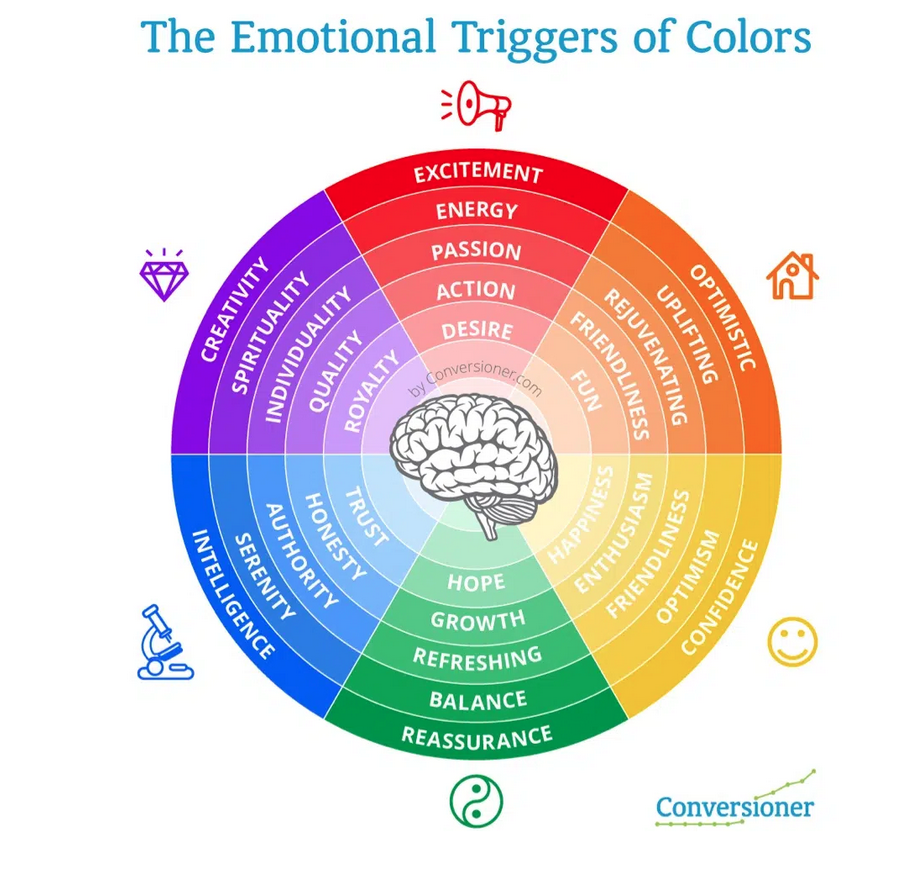
\includegraphics[width=0.8\textwidth]{bilder/farbkreis.png}
\caption{Ein aktueller Farbkreis (\cite{DesignEmo2003})}
\label{fig20:farbkreis}
\end{figure}\\

Die Wahl von geringen Kontrasten spielt ebenfalls eine wichtige Rolle bei der Schaffung einer gelassenheitserzeugenden Webseite. Hohe Kontraste können die Aufmerksamkeit des Benutzers stark beanspruchen und eine gewisse Unruhe verursachen. Indem man sich für geringere Kontraste entscheidet, schafft man eine harmonische und ausgewogene visuelle Erfahrung. Die Augen des Nutzers werden nicht durch starke Unterschiede zwischen den Farben belastet, sondern können sanft über die Webseite gleiten, was zu einem entspannten und angenehmen Surferlebnis führt.\\
Ein Kontrast von 6.37:1 ist niedrig. \\

% Contrastchecker
\begin{figure}[H]
    \centering
    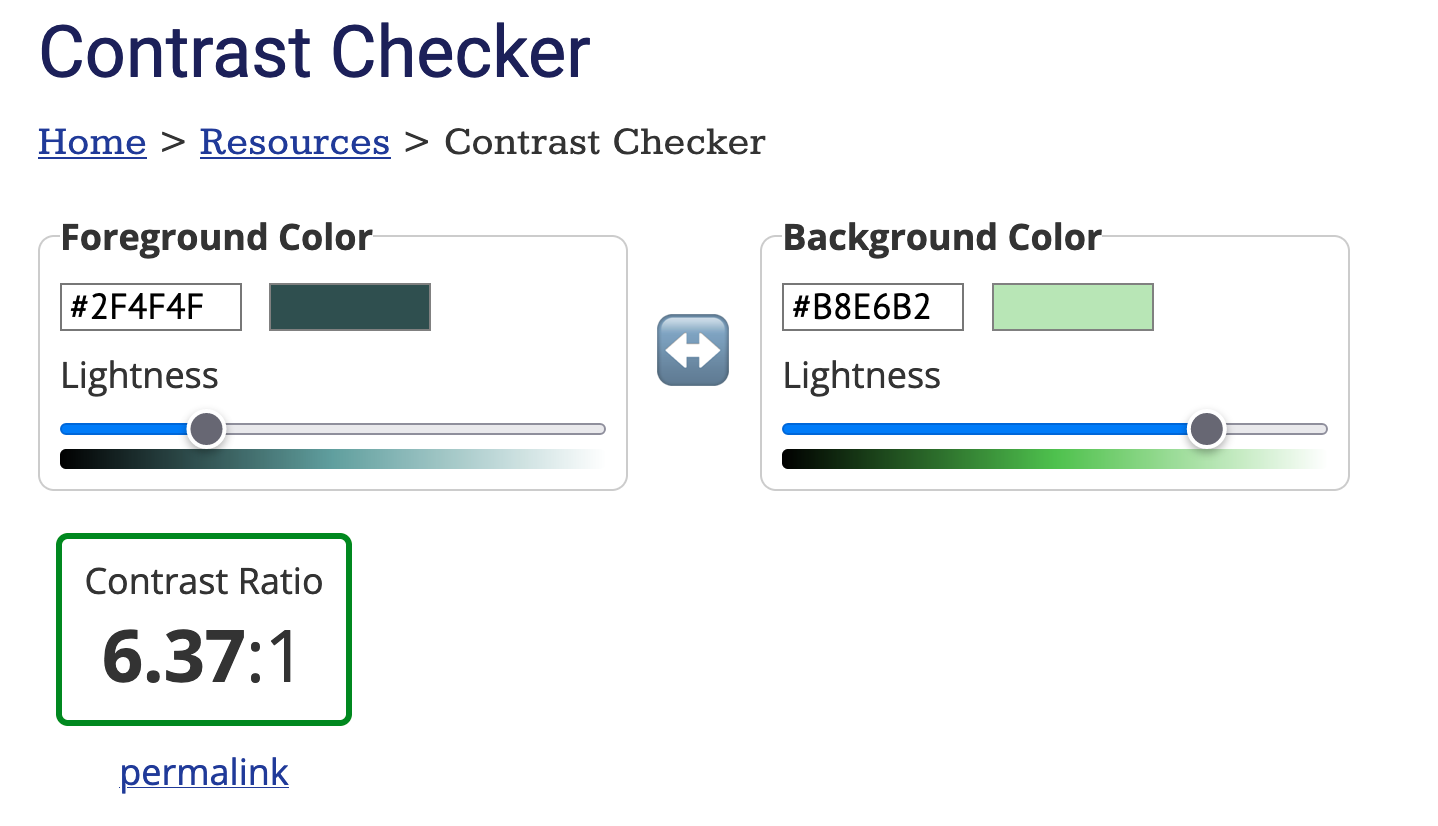
\includegraphics[width=0.8\textwidth]{bilder/contrast-gelassenheit.png}
    \caption{Das Kontrastverhältnis Schrift zu Hintergrund in dieser Anwendung}
    \label{fig21:contrast}
\end{figure}\\

\begin{figure}[H]
    \centering
    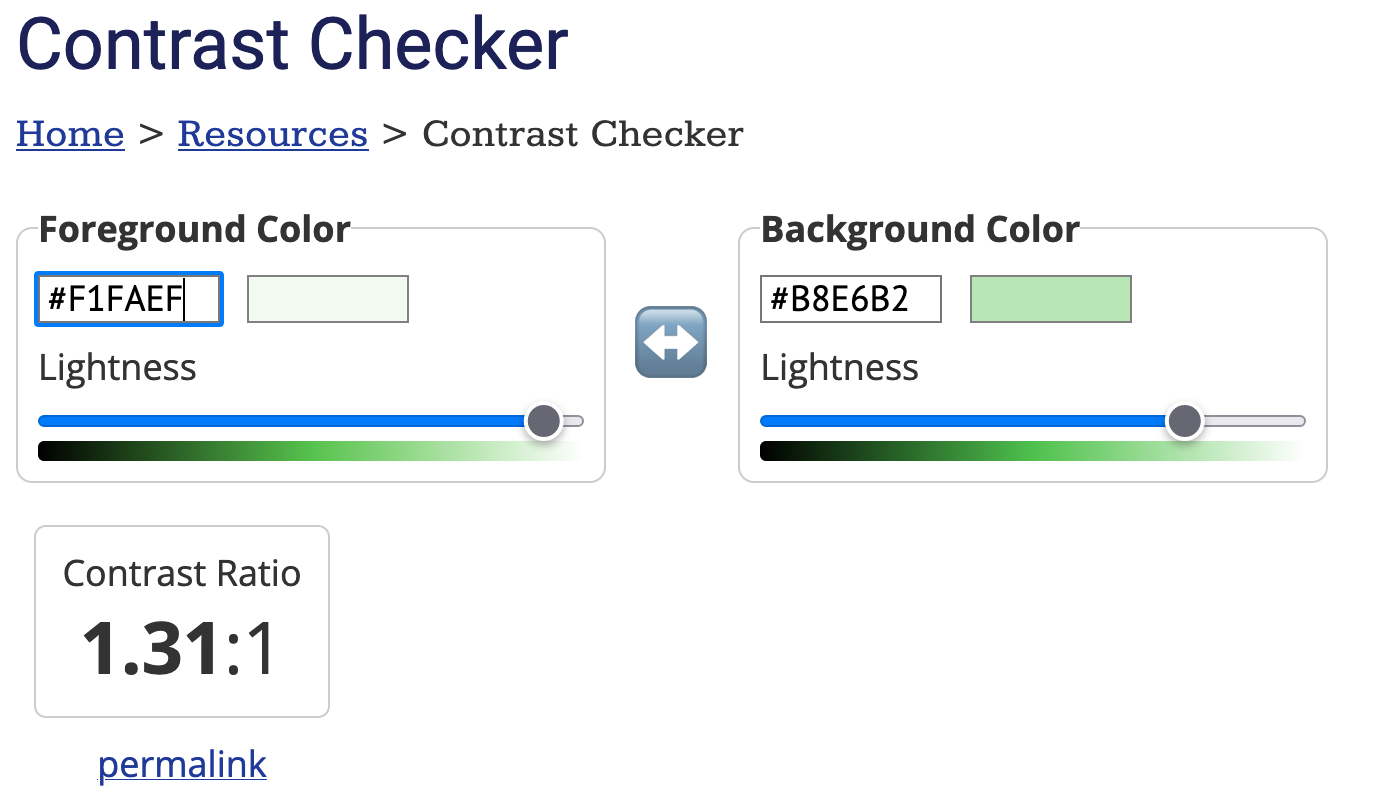
\includegraphics[width=0.8\textwidth]{bilder/contrast-box.png}
    \caption{Das Kontrastverhältnis Schrift zu Textbox in dieser Anwendung}
    \label{fig23:contrast}
\end{figure}\\

Des Weiteren ist die Reduktion ablenkender Elemente von großer Bedeutung, wenn es um die Erzeugung von Gelassenheit auf einer Webseite geht. Eine überladene und unübersichtliche Gestaltung kann den Nutzer überfordern und Stress verursachen. Durch die Reduktion von unnötigen visuellen Reizen kann der Fokus des Benutzers auf die wesentlichen Inhalte gelenkt werden. Dies fördert eine meditative Erfahrung und ermöglicht es dem Nutzer, sich auf das Wesentliche zu konzentrieren, ohne sich von irrelevanten Elementen ablenken zu lassen.\\

Die Kombination aus sanften Grüntönen, geringen Kontrasten und einer auf das Wesentliche reduzierten Gestaltung schafft also eine Webseite, die Gelassenheit und Entspannung fördert. Dies ist besonders relevant in einer Zeit, in der digitale Medien häufig mit stressigen und überwältigenden Erfahrungen in Verbindung gebracht werden. Eine gelassenheitserzeugende Webseite kann somit nicht nur das Wohlbefinden der Nutzer steigern, sondern auch eine positive Wahrnehmung und Bindung an die Webseite fördern.\\

% Farbpalette Adobe Color

\begin{figure}[H]
    \centering
    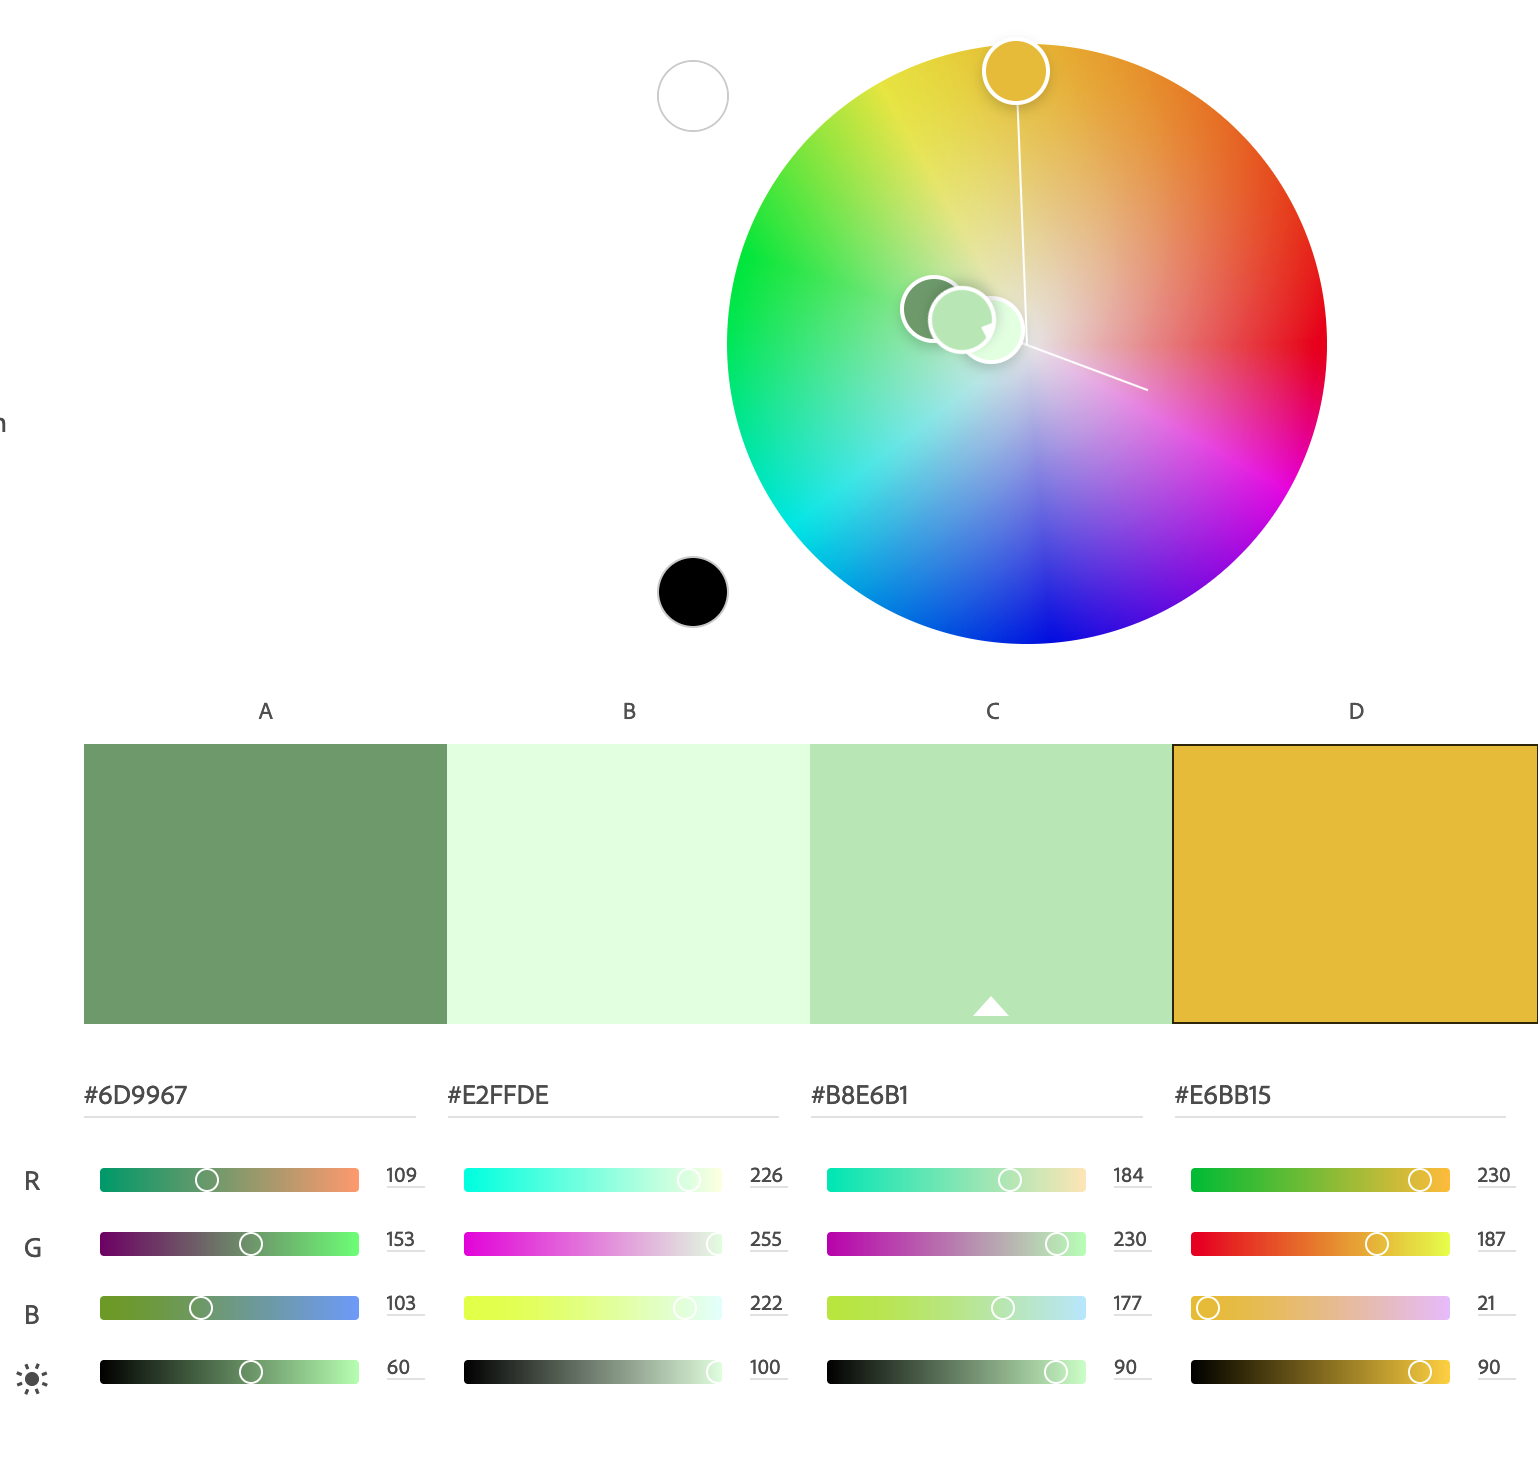
\includegraphics[width=0.8\textwidth]{bilder/adobecolor.png}
    \caption{Die gewählte Farbgestaltung}
    \label{fig22:adobecolor}
\end{figure}\\

Darüber hinaus wird durch Einhaltung des Gesetzes der Nähe eine leichte Orientierung ermöglicht.  Zusammenfassend lässt sich sagen, dass die bewusste Gestaltung von Webseiten durch die Wahl bestimmter Farben und Kontraste eine signifikante Auswirkung auf die emotionalen Zustände der Nutzer hat. Die gezielte Nutzung von sanften Grüntönen, geringen Kontrasten und einer reduzierten Gestaltung kann eine Atmosphäre der Gelassenheit schaffen und den Nutzern eine angenehme und entspannende Erfahrung bieten. Webseiten, die diese Gestaltungsprinzipien berücksichtigen, haben das Potenzial, eine nachhaltige und positive Wirkung auf das emotionale Wohlbefinden ihrer Besucher zu entfalten.\\

\begin{figure}[H]
    \centering
    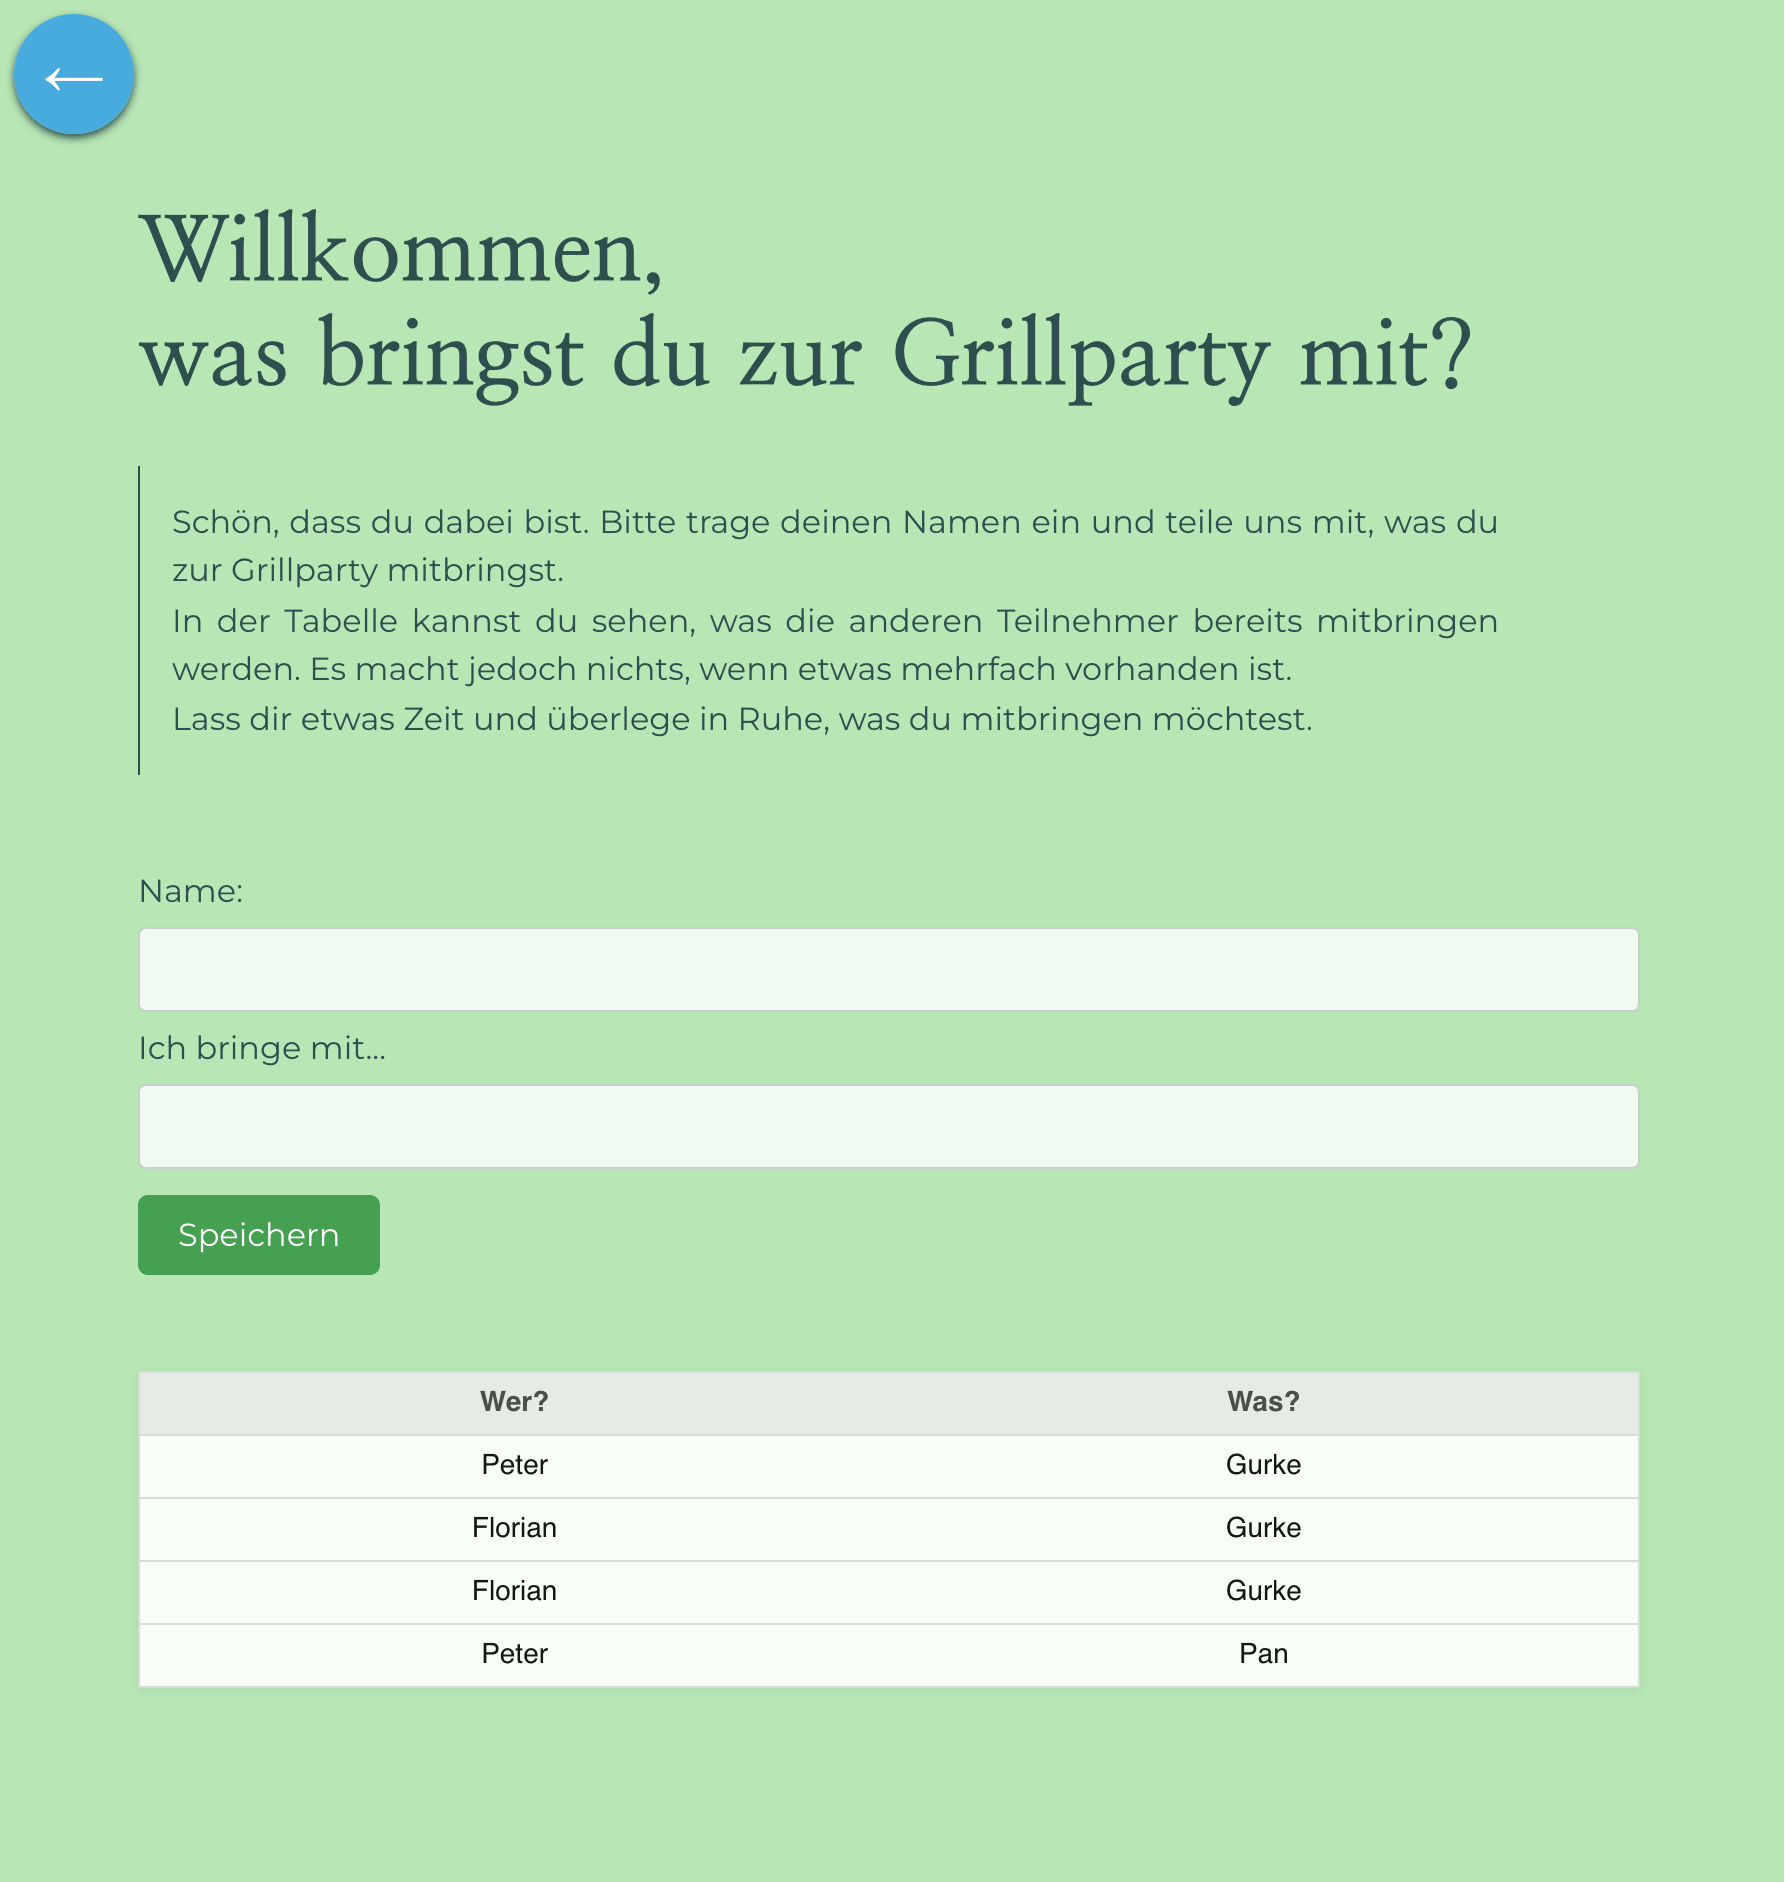
\includegraphics[width=0.8\textwidth]{bilder/website-gelassen.png}
    \caption{Die vollständige Website}
    \label{fig21:website-gelassen}
    \end{figure}\\

\begin{figure}[H]
        \centering
        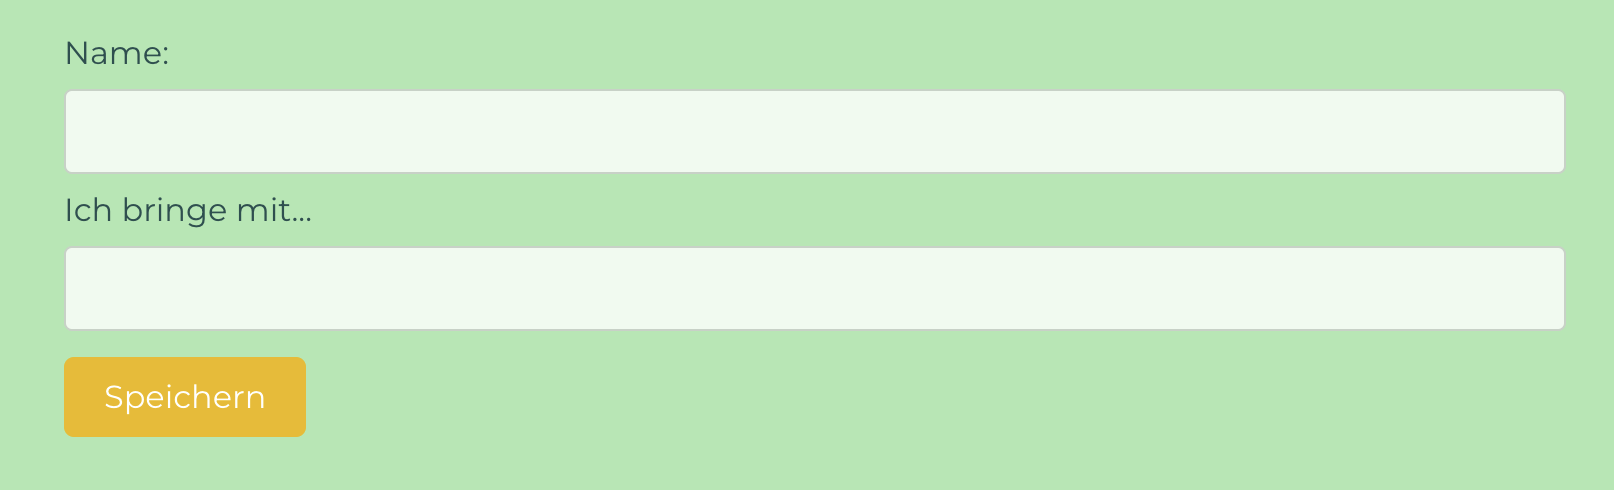
\includegraphics[width=0.8\textwidth]{bilder/website-gelassen-hover.png}
        \caption{Der Button wird bei Mouseover gelb}
        \label{fig22:website-gelassen-hover}
\end{figure}\\
    

\pagebreak
\section{Webseite - bewusstes Einsetzen der Elemente für die Induzierung von Nostalgie}
In diesem Teilprojekt lag der Fokus auf dem bewussten Einsatz von Medien und Gestaltungselementen aus vergangenen Ären. Wie im Kapitel „Emotionaler Einfluss von audiovisuellen Medien im Webdesign“ beschrieben, haben Musik und Geräusche einen erheblichen Einfluss auf die Induktion von Nostalgie, wie Smalley et al. (2023) festgestellt haben. Im Abschnitt „Emoticon Two“ der Website wurde daher ein Webdesign gewählt, das den Nutzer durch seine positive und gelassene Gestaltung in eine angenehme Grundstimmung versetzen soll. \\

Das Thema der gezielten Induktion von Nostalgie erfordert ein fundiertes Verständnis. Nur mit diesem Verständnis können Designelemente für eine Webseite, die explizit die Induktion von Nostalgie zum Ziel hat, adäquat ausgewählt und implementiert werden.

\subsection{Nostalgie als emotionales Korrektiv}
Nostalgie bezeichnet die empfundene Emotion als Reaktion auf die Erinnerung an spezifische Objekte, vergangene Lebensumstände, olfaktorische und akustische Reize sowie vertraute Praktiken. Solche Erinnerungen können zu einer intensiven Immersion in vergangene Episoden führen und ein anhaltendes Gefühl der Sehnsucht hervorrufen. In der wissenschaftlichen Literatur werden Personen, die solche Empfindungen häufig erleben, als "Nostalgiker" bezeichnet. \\

Die durch die Nostalgie hervorgerufenen Zustände können sowohl positive als auch negative Eigenschaften aufweisen, zeichnen sich jedoch stets durch eine hohe emotionale Intensität aus. Nostalgie wird in der akademischen Forschung unterschiedlich klassifiziert – mal als Emotion, mal als sehnsuchtsvolle Hinwendung (\cite{Hepper2011} ; \cite{Stangl2023}). Ursprünglich wurde Nostalgie im medizinischen Kontext verwendet, aber durch die evolutionäre Entwicklung der Psychologie und ihre wachsende Bedeutung in der modernen Gesellschaft hat sich die Wahrnehmung und Bedeutung dieses Begriffs gewandelt (\cite{Stangl2023}). Es ist wichtig zu beachten, dass die emotionale Codierung von Farben kulturspezifisch variiert. Daher wird Nostalgie in verschiedenen kulturellen Kontexten unterschiedlich interpretiert und erlebt (\cite{Roberson2006}).\\

\subsection{Umsetzung}

Für die Umsetzung der Nostalgie induzierenden Website, war es wichtig ein Motiv zu haben, das jeden Nutzer anspricht. Das standard Layout das die verwendeten HTML Klassen mit sich bringen, wurde deshalb an das veraltete Windows 98 Thema angepasst, um im Stil des vergangenen Kohärent zu bleiben. Weiter wurde als Hintergrund ein Bild gewählt, das desaturierte Farben besitzt und an alte Bücher oder Fotoalben erinnern soll. 

% Bild hintergrund
\begin{figure}[H]
    \centering
    
\includegraphics[width=0.8\textwidth]{bilder/hintergrund-scott.png}
    \caption{Das Hintergrundbild}
    \label{fig23:hintergrund}
\end{figure}\\


Nostalgie, als ein Gefühl der Sehnsucht nach vergangenen Zeiten, ist intrinsisch mit den individuellen Erfahrungen und Erinnerungen jeder Person verbunden. Diverse Artefakte – sei es in Form von Bildern, Videos oder Liedern – können abhängig von der Generation unterschiedliche emotionale Reaktionen hervorrufen. Ein prägnantes Beispiel hierfür wäre die Darstellung einer bekannten Persönlichkeit aus vergangenen Zeiten. Während diese Darstellung bei einigen Individuen nostalgische Gefühle auslösen kann, könnte sie für andere weniger relevant sein. Ein essentielles Element für das Auslösen von Nostalgie ist die Fähigkeit des Individuums, eine Verbindung zu vergangenen Erfahrungen herzustellen. Insbesondere, wenn das Publikum aus Personen mit unterschiedlichen kulturellen und zeitlichen Hintergründen besteht, kann die Induktion von Nostalgie variieren. \\

Vor diesem Hintergrund war es von Relevanz, einen Ansatz zu entwickeln, der sicherstellt, dass ein Großteil der Nutzer eine emotionale Verbindung zu den präsentierten Inhalten erlebt. Eine potenzielle Lösung wurde in der Integration eines Dropdown-Menüs im Begrüßungselement unserer digitalen Anwendung gefunden. Dieses Menü ermöglicht es dem Benutzer, eine spezifische Ära – wie die “70er, 80er, 90er oder 2000er” – auszuwählen. Auf Basis dieser Entscheidung wird dem Nutzer ein Inhalt präsentiert, der charakteristisch für die gewählte Epoche ist. Die von einem Nutzer ausgewählte Epoche könnte ein Zeichen für seine persönliche Präferenz sein, wodurch das zur Verfügung gestellte Material potentiell von Relevanz sein und in Folge dessen Nostalgie induzieren könnte. \\

% Bild Auswahl
\begin{figure}[H]
    \centering
    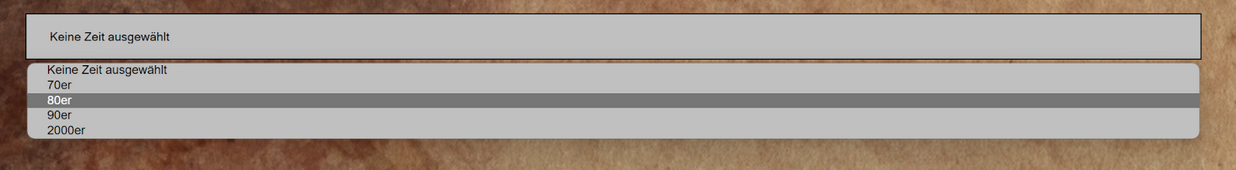
\includegraphics[width=0.8\textwidth]{bilder/dropdown-scott.png}
    \caption{Das Auswahlmenü}
    \label{fig23:auswahl}
\end{figure}\\


Die Rolle von akustischen Komponenten in der Nostalgie-Induzierung wurde durch Smalley et al. hervorgehoben. Weiter haben Xu et al. (2004) bereits auf die Bedeutung des Abstands der Schnitte und des Rhythmus in Bezug auf die Emotionsinduktion in audiovisuellen Inhalten verwiesen. Darüber hinaus hat Knautz (2010), gezeigt, dass Musik unabhängig von ihrer Epoche ein effektives Medium zur Emotionsinduktion ist. In Übereinstimmung mit ihren Erkenntnissen wurde die Verwendung von Musikvideos zur Nostalgie-Induktion gewählt, da diese beide Komponenten, akustische und visuelle, in sich vereinen. Außerdem bieten sie den zusätzlichen Vorteil, verschiedene Aspekte einer Ära einzufangen und somit das Potential zur Nostalgie-Induzierung zu maximieren. Musikvideos, die sowohl einen Song einer bestimmten Epoche als auch visuelle Elemente derselben Epoche enthalten, sind prädestiniert für eine Nostalgie induzierende Umgebung. Sie kombinieren typische Klangelemente mit charakteristischen visuellen Elementen dieser Ära. \\

Bei der Auswahl der Musikvideos wurden die bekanntesten und ikonischsten der jeweiligen Ära gewählt. Die Kriterien beinhalten die Popularität der Songs in den Genres Pop und Charts, da diese oft eine Kombination aus zeitgenössischem Charakter und emotionaler Tiefe bieten. Das Ziel war es, ein breites Spektrum an Hörern zu erreichen, um die Wahrscheinlichkeit der Nostalgie-Induktion zu maximieren. \\

% Bild 2 Screens
\begin{figure}[H]
    \centering
    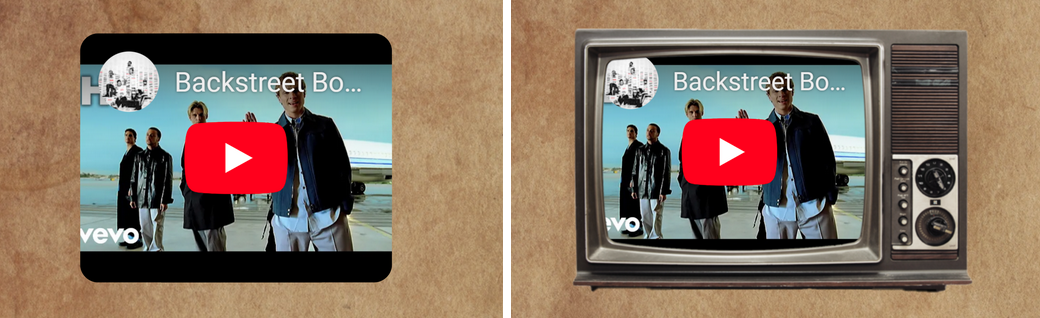
\includegraphics[width=0.8\textwidth]{bilder/auswahl-videos.png}
    \caption{Die Website mit Videos aus den Jahrzehnten}
    \label{fig22:youtube}
\end{figure}\\


Für eine angemessene Präsentation wurde der voreingestellte Stil zur Einbindung von Musikvideos im Browser, erweitert und in einem Bild eines alten Fernsehers dargestellt. Die Präsentation des Videos ohne den Fernseher stellt einen statischen Charakter dar und passt nicht in die Optik der Vergangenheit des Windows 98 Schemas.


\pagebreak
\section{Webseite - bewusstes Einsetzen von negativen Emotionen Stress - Unsicherheit - Angst}
Im folgenden Teilprojekt wurden bewusst eher negative Emotionen eingesetzt. Wie im theoretischen Teil dieser Arbeit beschrieben bürgen diese jedoch oftmals auch ein sehr hohes Motivationspotenzial, wodurch der Nutzer eher geneigt sein kann, eine Handlung auszuführen.\\
Auch Dominanz spielt dabei eine wichtige Rolle, wie beschrieben, führt diese typischerweise eher zu hoher Erregung und zu hoher Motivation. Dies wird durch folgende Gestaltung erreicht:\\
Harte Kanten, eckige Formen. Dies zeigt sich in den verwendeten Input-Feldern und dem eckigen Button. Auch die Schriftart ist sehr klar gehalten. Zusätzlich dazu wurden sehr harte Kontraste gewählt, die Trennung zwischen dem Schwarzen Hintergrund und den weißen Texten und Inputfeldern ist sehr stark.

\begin{figure}[H]
    \centering
    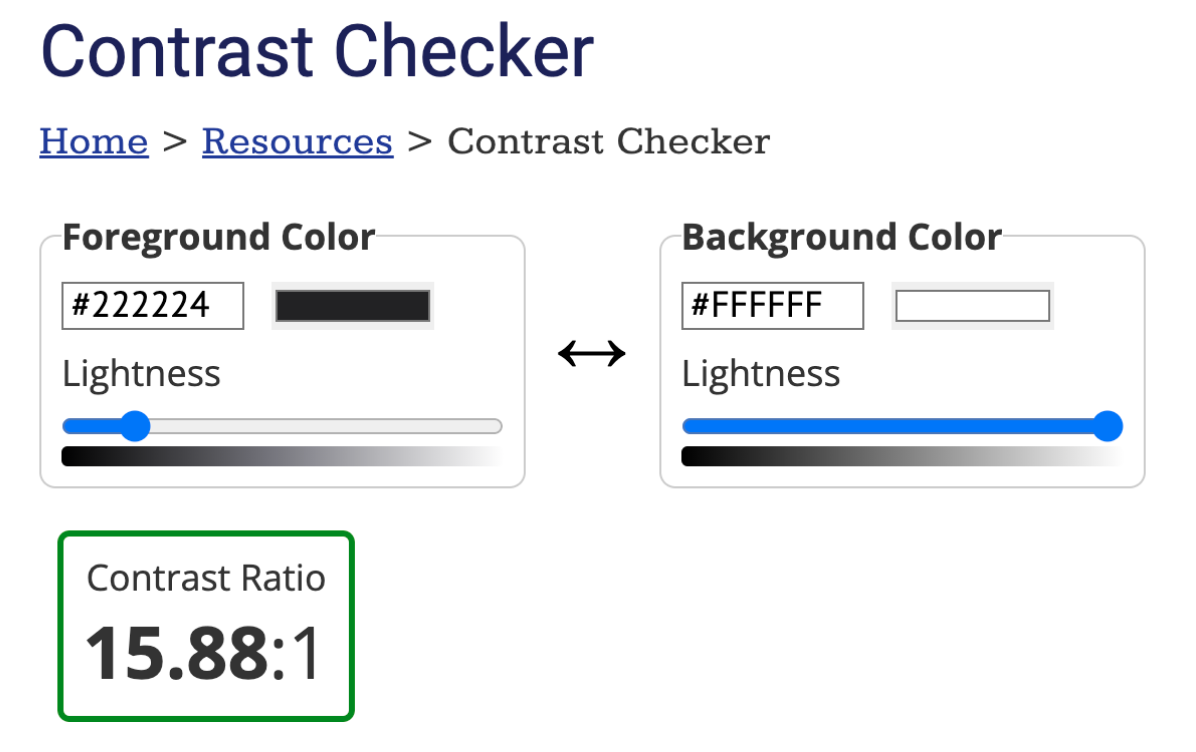
\includegraphics[width=0.8\textwidth]{bilder/contrast.png}
    \caption{Starke Kontraste} % TODO
    \label{fig12:contrast}
\end{figure}\\

\begin{figure}[H]
    \centering
    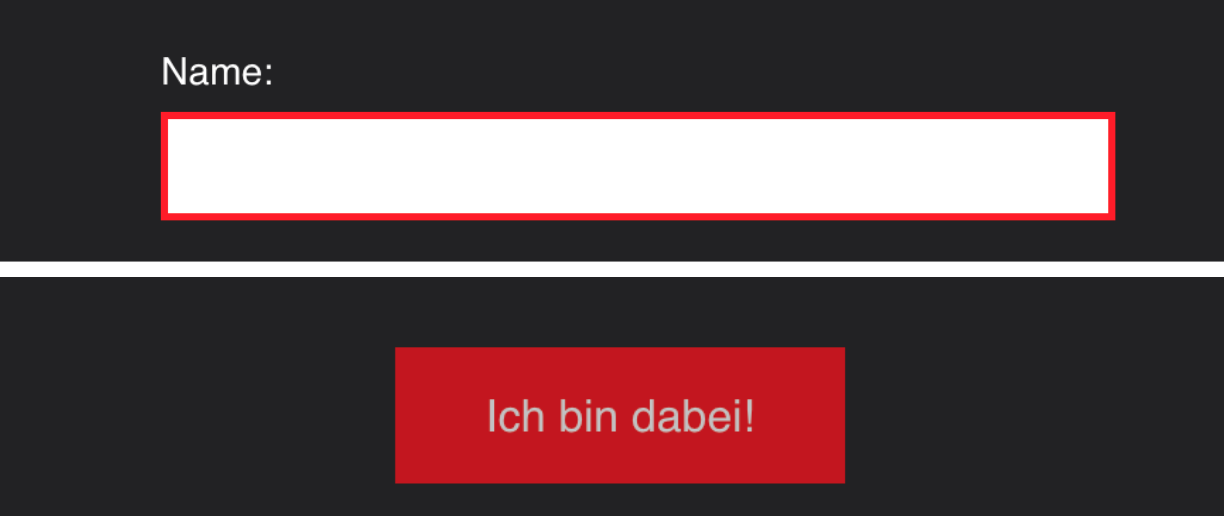
\includegraphics[width=0.8\textwidth]{bilder/name-bin-dabei.png}
    \caption{Eintragen des Namens und Submit-Button} % TODO
    \label{fig13:name}
\end{figure}\\

\subsection{Stress}
Um den Nutzer unter Druck zu setzen und ein Handeln zu forcieren, wurden hauptsächlich Blink-Effekte eingesetzt. Zusätzlich dazu wurde auch durch Storytelling, mit dem Hinweis, dass nur noch wenige Plätze verfügbar sind, Druck auf den Nutzer aufgebaut. Durch den Timer wird er weiter Stress ausgesetzt, der Druck wird durch das schrittweise Vergrößern der Schriftgröße zusätzlich unterstützt.\\
Im folgenden Screenshot sieht man den rot blinkenden Text, der darauf aufmerksam macht, dass nur noch 3 Plätze frei sind. Somit soll ein schnelles handeln erzwungen werden, bevor womöglich alle Plätze vergeben sind. Die rote Farbe als Signalfarbe deutet zusätzlich darauf hin, dass hier erhöhte Aufmerksamkeit gefordert ist.\\


\begin{figure}[H]
    \centering
    \includegraphics[width=0.8\textwidth]{bilder/schrift-freie-plätze3.png}
    \caption{Herabzählen der Anzeige erzeugt Stress}
    \label{fig14:platz}
\end{figure}\\


Mit Ablaufen des Timers vergrößert sich auch die Schrift. Dadurch wird noch mehr Aufmerksamkeit erzwungen und der Nutzer weiter unter Druck gesetzt.\\
Der Text zählt zunächst weiter runter und endet dann bei einem blinkenden “nur noch EIN Platz frei”, was suggeriert, dass nun endgültig gehandelt werden muss, bevor alle Plätze vergeben sind. Dies wird zusätzlich dadurch unterstützt, dass nun auch alle Input-Felder mit einem roten blinkenden Rahmen ausgestattet werden, sollten sie noch nicht ausgefüllt worden sein. \\


\begin{figure}[H]
    \centering
    \includegraphics[width=0.8\textwidth]{bilder/schrift-freie-plätze1.png}
    \caption{Herabzählen der Anzeige erzeugt Stress}
    \label{fig14:platz1}
\end{figure}\\

Auch der submit-button übernimmt den leuchtend roten, blinkenden Stil, wenn die Inputfelder erfolgreich ausgefüllt wurden und setzt den Nutzer unter Stress, um ein Handeln zu erzwingen.

% Bild button

\begin{figure}[H]
    \centering
    
\includegraphics[width=0.8\textwidth]{bilder/rot-dabei.png}
    \caption{Rot leuchtender Submit-Button}
    \label{fig15:submit}
\end{figure}\\


\subsection{Unsicherheit}

\begin{figure}[H]
    \centering
    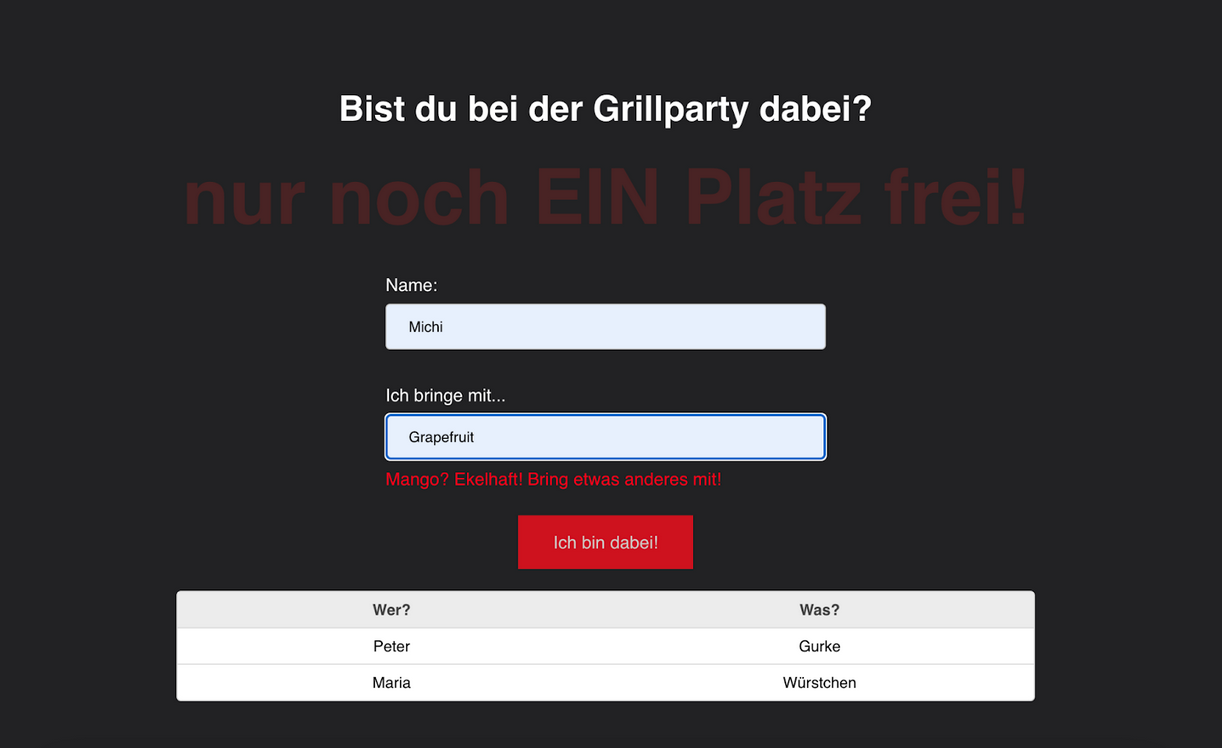
\includegraphics[width=0.8\textwidth]{bilder/ekelhaft.png}
    \caption{Unfreundliche Kommunikation} %% TODO
    \label{fig16:ekel}
\end{figure}\\


\begin{figure}[H]
    \centering
    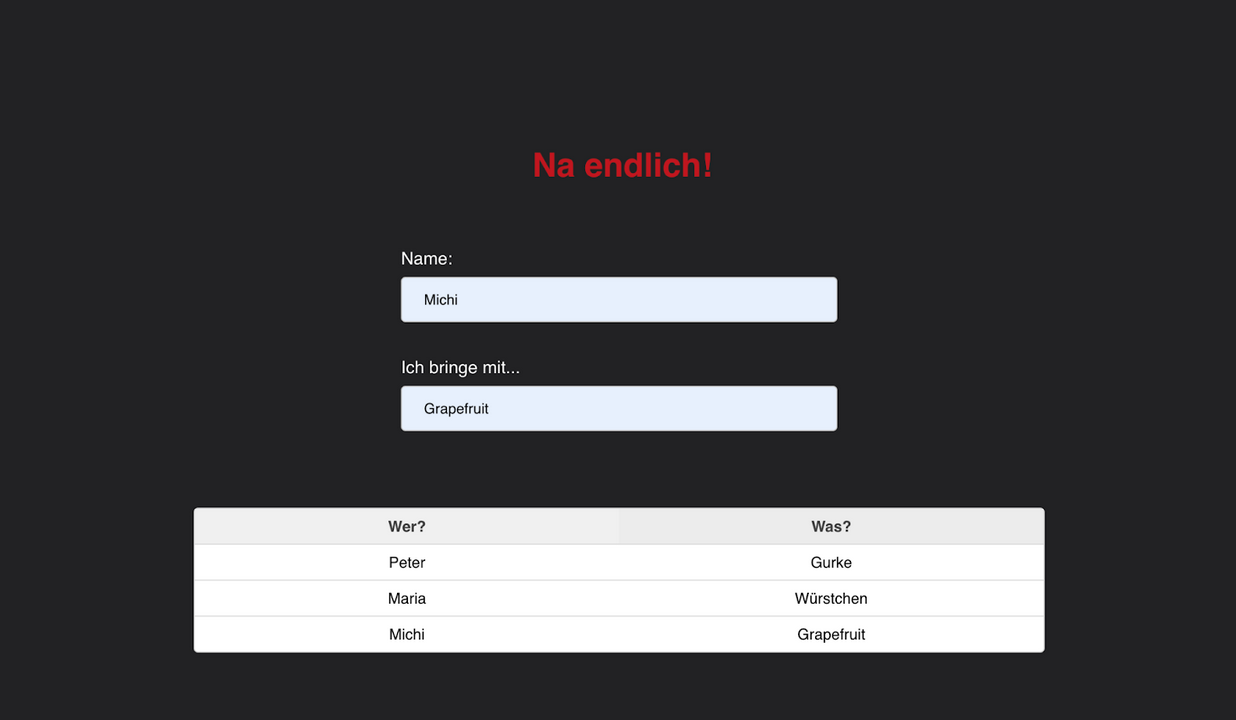
\includegraphics[width=0.8\textwidth]{bilder/na-endlich.png}
    \caption{Letztlich wird die Eintragung vorgenommen}
    \label{fig17:okay}
\end{figure}\\


\subsection{Angst}
Auch Angst als sehr starke Emotion  kann genutzt werden, um Handlungen zu forcieren. Hierbei muss man auch aufpassen, dass diese nicht zu stark ist, sodass der Nutzer noch handlungsfähig ist. Wird Angst richtig dosiert, kann sie dazu beitragen, dass sich Botschaften beim Nutzer besser einprägen. Im Beispiel der hier betrachteten Webseite wird diese durch die dunklen Farben unterstützt und die Darstellung des angstvollen/aufmerksamen Gesichts (insbesondere Augenpartie), das sehr groß auf der Webseite dargestellt ist und zusätzlich durch die Animation der Augen Aufmerksamkeit generiert. Somit soll der Nutzer animiert werden, auch wirklich zu der Grillparty zu kommen.\\

\begin{figure}[H]
    \centering
    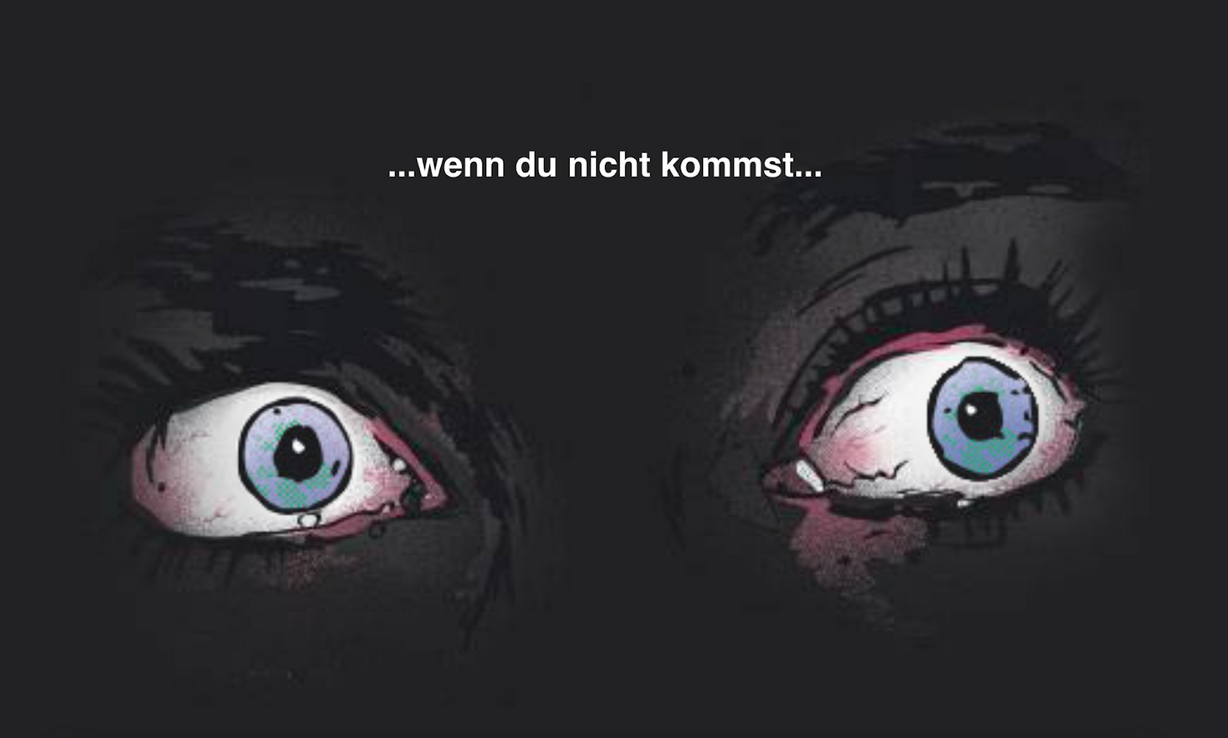
\includegraphics[width=0.8\textwidth]{bilder/angst1.png}
    \caption{Bewusstes erzeugen von Angst}
    \label{fig18:angst1}
\end{figure}\\

\begin{figure}[H]
    \centering
    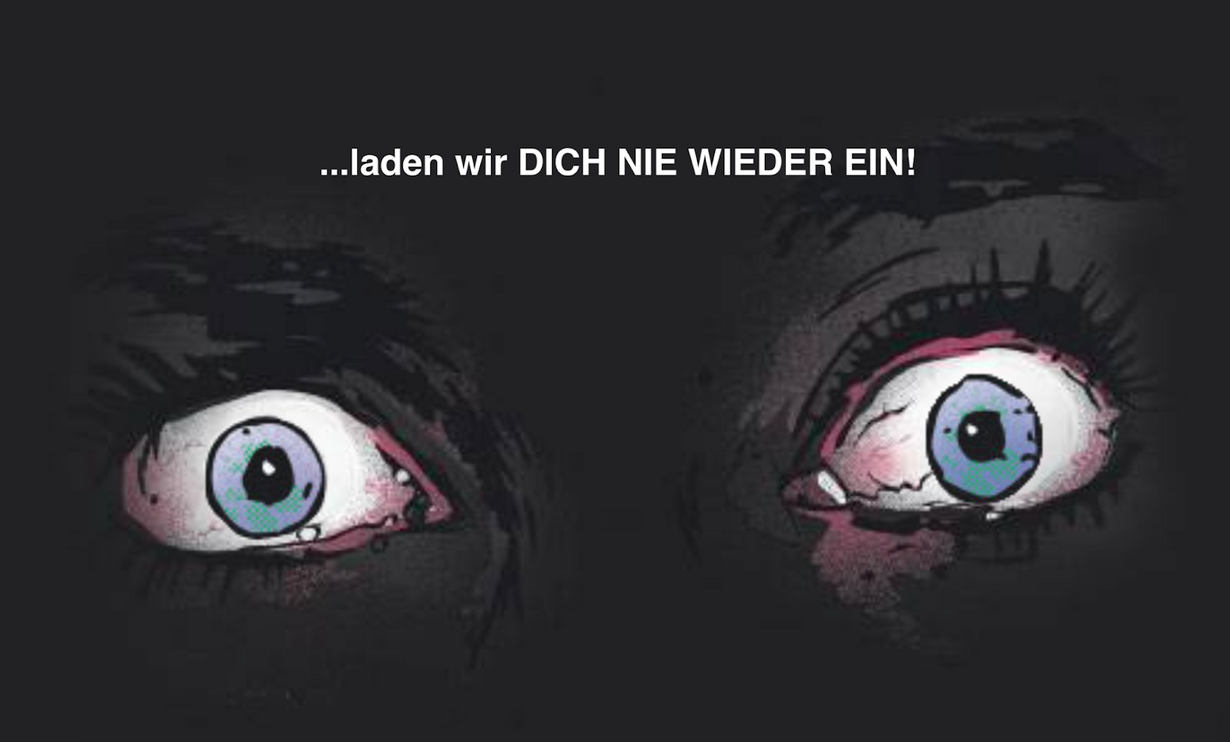
\includegraphics[width=0.8\textwidth]{bilder/angst2.png}
    \caption{Bewusstes erzeugen von Angst}
    \label{fig19:angst2}
\end{figure}\\

\section{Implikationen}
\subsection{Sprachliche Relativität}
In Anbetracht der Gestaltung der Website, ist die Sapir-Whorf-These zu benennen. Laut dieser These kann die Art und Weise, wie wir denken, durch die semantische Struktur unserer Sprache divergieren (\cite{Cibelli2016}). Eine Abgeleitete Hypothese von Roberson et. al (2006) hat dafür weitere Hinweise festgestellt. So soll ein indigener Stamm aus Namibia mit dem Test aus Abbildung X konfrontiert worden sein. Die Zielgruppe wurde dazu aufgefordert das Quadrat zu finden, das nicht die gleiche Farbe hat wie der Rest. Bei dem ersten Test wurden alle Farben als gleich betitelt, es konnte kein andersfarbiges Quadrat festgestellt werden. Bei dem zweiten Test hingegen wurde ein Unterschied festgestellt. Beachtlich ist dies, da der Kontrast aus dem ersten Test verglichen mit dem des 2. Test deutlich erkennbar  ist, für Individuen unseres Kulturkreises.\\
In dieser Arbeit wir also die emotionale Wirksamkeit bestimmter Gestaltungselemente unseren Kulturkreises berücksichtigt und ist somit nicht anwendbar auf die gesamte Bevölkerung. 


\end{document}


